\section{Implementierung}

\subsection{Umgesetzt}
\begin{frame}
	\frametitle{Mitwirkung}
	
	Implementierung der Inhalte für:
	\begin{enumerate}
		\item Gästebuch
		\item Top-Gästebuch
		\item Nachrichten
		\item Adminverwaltung
		\begin{itemize}
			\item Nachrichteneinträge löschen
		\end{itemize}
		\item Statische Inhalte
		\begin{itemize}
			\item Unternehmen
			\item Kontakt
			\item AGB
			\item Impressum
		\end{itemize}
	\end{enumerate}
\end{frame}

\subsubsection{Gästebuch}

\begin{frame}
\begin{figure}
\frametitle{Ansicht - Gästebuch}
\centering
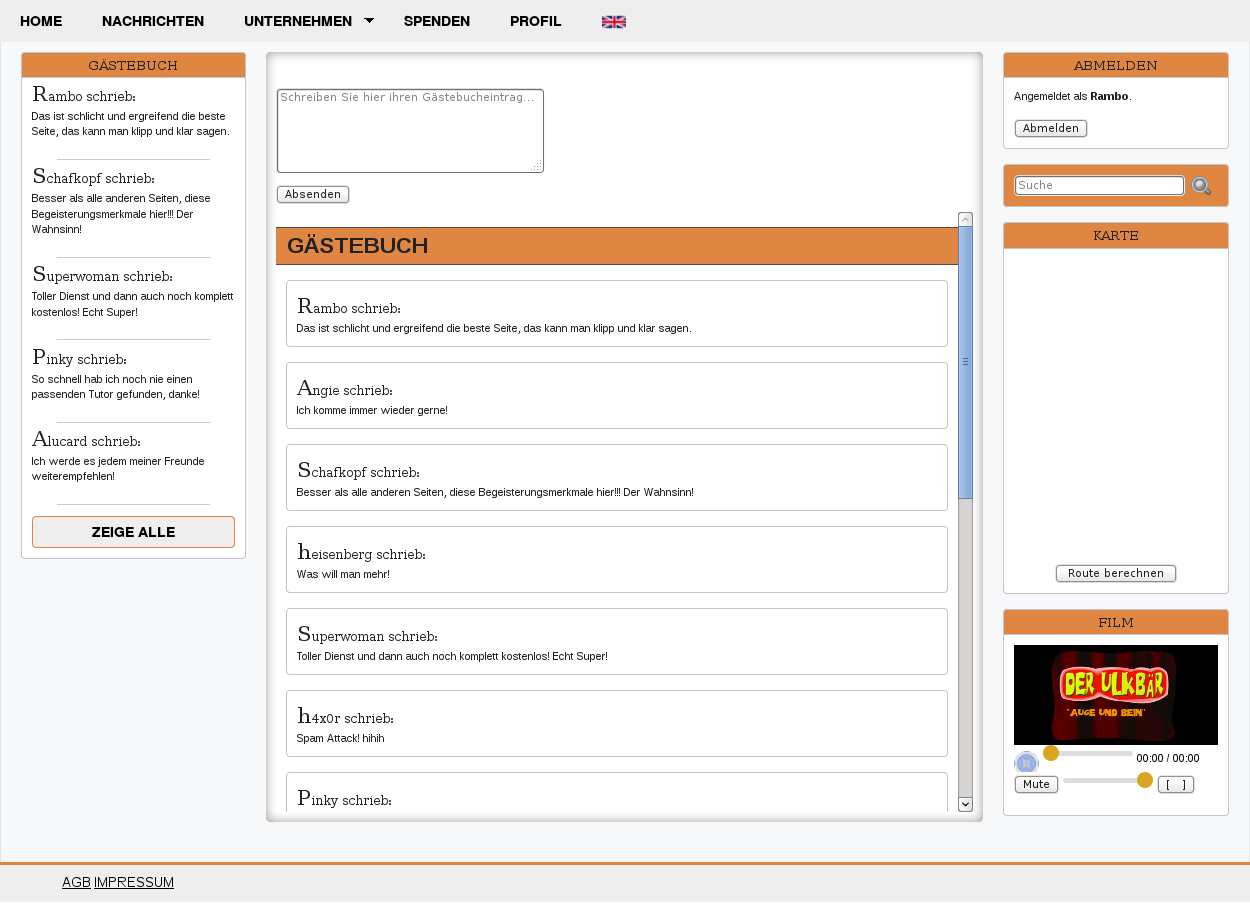
\includegraphics[width=0.85\linewidth]{./Source/Gaestebuch_logged_in}
%\caption{Gästebuch + Top-Gästebuch}
\label{fig:Gaestebuch}
\end{figure}


\end{frame}


\defverbatim[colored]
\makeset{
%%%%%%%%%%%%%%%%%%% PHP SUPPORT %%%%%%%%%%%%%%%%%%%%%%%%
\definecolor{dkgreen}{rgb}{0,.6,0}
\definecolor{dkblue}{rgb}{0,0,.6}
\definecolor{dkyellow}{cmyk}{0,0,.8,.3}

\lstset{
  language        = php,
  backgroundcolor=\color{lightgray},
  extendedchars=true,
  basicstyle=\tiny\ttfamily,
  showstringspaces=false,
  showspaces=false,
  numbers=left,
  numberstyle=\tiny\ttfamily,
  numbersep=9pt,
  tabsize=2,
  breaklines=true,
  showtabs=false,
  frame=leftline,
  keywordstyle    = \color{dkblue},
  stringstyle     = \color{red},
  identifierstyle = \color{dkgreen},
  commentstyle    = \color{gray},
  emph            =[1]{php},
  emphstyle       =[1]\color{black},
  emph            =[2]{if,and,or,else},
  emphstyle       =[2]\color{dkyellow}
  }
  
gaestebuch.php
\begin{lstlisting}[language=php]
<form name="addguestbookentry" method="post" action="/scripts/WriteGuestbook.php" id="gbform">
    <input type="hidden" name="sprache" value="<?php echo $_SESSION['sprache']; ?>">
    <input type="hidden" name="username" value="<?php echo $_SESSION['user']; ?>">
    <div>
        <label for ="nachrichtentext"></label>
        <p>
            <textarea name="eintrag" cols="33" rows="5" maxlength="300" id="nachrichtentext" placeholder ="Schreiben Sie hier ihren Gaestebucheintrag..." required></textarea>
        </p>
    </div>
    <div class="line submit">
        <input type="submit" value="Absenden">
    </div>
</form>
\end{lstlisting}
  
gaestebuch.html
\begin{lstlisting}[language=html]
<h1>G&auml;stebuch</h1>
<p id="data"></p>
<script type="text/javascript" src="/js/guestbook.js"></script>
\end{lstlisting}

}
\begin{frame} %%Eine Folie
  \frametitle{Gästebucheinträge - Teil 1} %%Folientitel
  \makeset
\end{frame}

\defverbatim[colored]
\makeset{
%%%%%%%%%%%%%%%%%%% PHP SUPPORT %%%%%%%%%%%%%%%%%%%%%%%%
\definecolor{dkgreen}{rgb}{0,.6,0}
\definecolor{dkblue}{rgb}{0,0,.6}
\definecolor{dkyellow}{cmyk}{0,0,.8,.3}

\lstset{
  language        = php,
  backgroundcolor=\color{lightgray},
  extendedchars=true,
  basicstyle=\tiny\ttfamily,
  showstringspaces=false,
  showspaces=false,
  numbers=left,
  numberstyle=\tiny\ttfamily,
  numbersep=9pt,
  tabsize=2,
  breaklines=true,
  showtabs=false,
  frame=leftline,
  keywordstyle    = \color{dkblue},
  stringstyle     = \color{red},
  identifierstyle = \color{dkgreen},
  commentstyle    = \color{gray},
  emph            =[1]{php},
  emphstyle       =[1]\color{black},
  emph            =[2]{if,and,or,else},
  emphstyle       =[2]\color{dkyellow}
  }
  

guestbook.js
\begin{lstlisting}[name=guestbook.js]
$(document).ready(function myFunction() {
    $.ajaxSetup({cache: false});
    var url = "/scripts/ReadGuestbook.php";

    $.ajax(    {
        type: 'post',
        url: url,
        dataType: 'json',
        cache: false,
        success: function(data)
        {
            var SingleEntry = new Array(data.length);

            for (var i = 0; i < data.length; i++)
            {
                SingleEntry.push("<div class='basic-wrapper'><div class=' GBauthor'>" + data[i]['benutzername'] + "</div><div class=' GBmessage'>" + data[i]['eintrag'] + "</div></div>");
            }

            var AllEntries = SingleEntry.join('');
            document.getElementById("data").innerHTML = AllEntries;
        }
    });
});
\end{lstlisting}


}
\begin{frame} %%Eine Folie
  \frametitle{Gästebucheinträge - Teil 2} %%Folientitel
  \makeset
\end{frame}

%\subsubsection{Nachrichten}
%
%\defverbatim[colored]
%\makeset{
%%%%%%%%%%%%%%%%%%%% PHP SUPPORT %%%%%%%%%%%%%%%%%%%%%%%%
%\definecolor{dkgreen}{rgb}{0,.6,0}
%\definecolor{dkblue}{rgb}{0,0,.6}
%\definecolor{dkyellow}{cmyk}{0,0,.8,.3}
%
%\lstset{
%  language        = php,
%  backgroundcolor=\color{lightgray},
%  extendedchars=true,
%  basicstyle=\tiny\ttfamily,
%  showstringspaces=false,
%  showspaces=false,
%  numbers=left,
%  numberstyle=\tiny\ttfamily,
%  numbersep=9pt,
%  tabsize=2,
%  breaklines=true,
%  showtabs=false,
%  frame=leftline,
%  keywordstyle    = \color{dkblue},
%  stringstyle     = \color{red},
%  identifierstyle = \color{dkgreen},
%  commentstyle    = \color{gray},
%  emph            =[1]{php},
%  emphstyle       =[1]\color{black},
%  emph            =[2]{if,and,or,else},
%  emphstyle       =[2]\color{dkyellow}
%  }
%  
%
%ReadNewsDelete.php
%\begin{lstlisting}[language=php]
%<?php
%	 include_once($_SERVER["DOCUMENT_ROOT"] . "/test_02/scripts/ConToDB.php");       // Inkludiert die Funktion zur Anmeldung an der DB
%    // Baue Verbindung auf
%    try 
%	{
%        $dbConnection = ConnectToDB();
%    } catch (Exception $e)
%	{
%        die("keine Verbindung moeglich: " . $e->getMessage());
%    }
%	$query = $dbConnection->prepare("SELECT * FROM news where 1 order by id desc");
%	if($query->execute() )
%		$result = $query->fetchAll(PDO::FETCH_ASSOC);
%		
%	$dbConnection = null;
%?>
%\end{lstlisting}
%}

%\begin{frame} %%Eine Folie
%  	\frametitle{Nachrichten - Teil 1} %%Folientitel
%	\makeset
%
%\end{frame}
%
%\defverbatim[colored]
%\makeset{
%%%%%%%%%%%%%%%%%%%% PHP SUPPORT %%%%%%%%%%%%%%%%%%%%%%%%
%\definecolor{dkgreen}{rgb}{0,.6,0}
%\definecolor{dkblue}{rgb}{0,0,.6}
%\definecolor{dkyellow}{cmyk}{0,0,.8,.3}
%
%\lstset{
%  language        = php,
%  backgroundcolor=\color{lightgray},
%  extendedchars=true,
%  basicstyle=\tiny\ttfamily,
%  showstringspaces=false,
%  showspaces=false,
%  numbers=left,
%  numberstyle=\tiny\ttfamily,
%  numbersep=9pt,
%  tabsize=2,
%  breaklines=true,
%  showtabs=false,
%  frame=leftline,
%  keywordstyle    = \color{dkblue},
%  stringstyle     = \color{red},
%  identifierstyle = \color{dkgreen},
%  commentstyle    = \color{gray},
%  emph            =[1]{php},
%  emphstyle       =[1]\color{black},
%  emph            =[2]{if,and,or,else},
%  emphstyle       =[2]\color{dkyellow}
%  }
%  
%
%admin.php
%\begin{lstlisting}[language=php]
%if(isset($_GET['deleteNews']) and $_GET['deleteNews'] == true) {
%	if(isset($_GET['fired']) and $_GET['fired'] == true and isset($_POST["NewsID"])){
%		$deleteNews = $_POST["NewsID"];
%		include_once($_SERVER["DOCUMENT_ROOT"] . "/test_02/scripts/DeleteNewsfromAdmin.php");
%	}
%	include_once($_SERVER["DOCUMENT_ROOT"] . "/test_02/scripts/ReadNewsDelete.php");
%	$newsresults = $result;
%	$news_print = "";
%	foreach($newsresults as $eintrag) {
%		$news_print .= "<tr> ";
%		$news_print .= "<th><div class='NewsDelEntry'> " . $eintrag["nachricht"] . "</div></th>";
%		$news_print .= "<th><div class='NewsDelTopic'> " . $eintrag["betreff"] . "</div></th>";
%		$news_print .= "<th><div class='NewsDelAuthor'> ". $eintrag["benutzername"] . "</div></th> ";
%		$news_print .= '<th><div class="NewsCheckbox"><input type="checkbox" name="NewsID[]" value="'. $eintrag["id"] . '"></div></th>';
%		$news_print .= "</tr>";
%	}
%	include_once($_SERVER["DOCUMENT_ROOT"] . "/test_02/de/content/ShowNewstoDelete.html");	
%}
%\end{lstlisting}
%}
%\begin{frame} %%Eine Folie
%  	\frametitle{Nachrichten - Teil 2} %%Folientitel
%	\makeset
%
%\end{frame}


\subsubsection{Statische Inhalte}
\defverbatim[colored]
\makeset{
%%%%%%%%%%%%%%%%%%% PHP SUPPORT %%%%%%%%%%%%%%%%%%%%%%%%
\definecolor{dkgreen}{rgb}{0,.6,0}
\definecolor{dkblue}{rgb}{0,0,.6}
\definecolor{dkyellow}{cmyk}{0,0,.8,.3}

\lstset{
  language        = php,
  backgroundcolor=\color{lightgray},
  extendedchars=true,
  basicstyle=\tiny\ttfamily,
  showstringspaces=false,
  showspaces=false,
  numbers=left,
  numberstyle=\tiny\ttfamily,
  numbersep=9pt,
  tabsize=2,
  breaklines=true,
  showtabs=false,
  frame=leftline,
  keywordstyle    = \color{dkblue},
  stringstyle     = \color{red},
  identifierstyle = \color{dkgreen},
  commentstyle    = \color{gray},
  emph            =[1]{php},
  emphstyle       =[1]\color{black},
  emph            =[2]{if,and,or,else},
  emphstyle       =[2]\color{dkyellow}
  }
  
kontakt.html
\begin{lstlisting}[language=html]
<h1>Kontakt:</h1>
<table>
<tr>
<td><p>Telefon:</p></td>
<td><p>0123456789</p></td>
</tr>
<tr>
<td><p>E-Mail:</p></td>
<td><p><a href="mailto:support@tutoren-ag.de">An den Support wenden</a></p></td>
</tr>
</table>
Unser Support ist taeglich 24h zu erreichen.<br>
\end{lstlisting}

}

\begin{frame} %%Eine Folie
  	\frametitle{Statische Inhalte - Beispiel: Kontakt} %%Folientitel
	\makeset

\end{frame}

\subsection{Nicht umgesetzt}

\begin{frame} %%Eine Folie
	\frametitle{Nicht umgesetzt} %%Folientitel

	Aus Zeitgründen konnten folgende Features nicht umgesetzt werden:
	\begin{enumerate}
		\item Punkt F17: Preismodell und Zahlungsinfos
		\newline Stattdessen wurde eine Spendenseite eingerichtet
		\item Punkt F42: Eigenes Schwarzes Brett für Tutoren
		\item Punkt F24/F34/F43: Zugriff aufs Nachrichtensystem
		\item Beurteilungen schreiben
	\end{enumerate}

\end{frame}

\subsection{Demonstration}

\begin{frame}
  \textbf{Es folgt eine Demonstration ...}
\end{frame}

%\begin{frame}
%  \frametitle{Ende}
%  \center
% \textbf{{Vielen Dank für Ihre Aufmerksamkeit}}
%\end{frame}